%%
%% This is file `sample-sigconf.tex',
%% generated with the docstrip utility.
%%
%% The original source files were:
%%
%% samples.dtx  (with options: `sigconf')
%% 
%% IMPORTANT NOTICE:
%% 
%% For the copyright see the source file.
%% 
%% Any modified versions of this file must be renamed
%% with new filenames distinct from sample-sigconf.tex.
%% 
%% For distribution of the original source see the terms
%% for copying and modification in the file samples.dtx.
%% 
%% This generated file may be distributed as long as the
%% original source files, as listed above, are part of the
%% same distribution. (The sources need not necessarily be
%% in the same archive or directory.)
%%
%% The first command in your LaTeX source must be the \documentclass command.
\documentclass[sigconf]{acmart}
\usepackage[ruled,vlined]{algorithm2e}
\SetKw{KwBy}{by}

%%
%% \BibTeX command to typeset BibTeX logo in the docs
\AtBeginDocument{%
  \providecommand\BibTeX{{%
    \normalfont B\kern-0.5em{\scshape i\kern-0.25em b}\kern-0.8em\TeX}}}

%% Rights management information.  This information is sent to you
%% when you complete the rights form.  These commands have SAMPLE
%% values in them; it is your responsibility as an author to replace
%% the commands and values with those provided to you when you
%% complete the rights form.
\setcopyright{acmcopyright}
\copyrightyear{2020}
\acmYear{2020}
\acmDOI{10.1145/1122445.1122456}

%% These commands are for a PROCEEDINGS abstract or paper.
\acmConference[MemSys '20]{MemSys '20: {Sept 28--Oct 01, 2020}{Washington, DC}}
\acmBooktitle{MemSys '20: MemSys, Sept 28--Oct 01, 2020, Washington, DC}
\acmPrice{15.00}
\acmISBN{978-1-4503-XXXX-X/18/06}


%%
%% Submission ID.
%% Use this when submitting an article to a sponsored event. You'll
%% receive a unique submission ID from the organizers
%% of the event, and this ID should be used as the parameter to this command.
%%\acmSubmissionID{123-A56-BU3}

%%
%% The majority of ACM publications use numbered citations and
%% references.  The command \citestyle{authoryear} switches to the
%% "author year" style.
%%
%% If you are preparing content for an event
%% sponsored by ACM SIGGRAPH, you must use the "author year" style of
%% citations and references.
%% Uncommenting
%% the next command will enable that style.
%%\citestyle{acmauthoryear}

%%
%% end of the preamble, start of the body of the document source.
\begin{document}

%%
%% The "title" command has an optional parameter,
%% allowing the author to define a "short title" to be used in page headers.
\title{CircusTent: A Benchmark Suite for Atomic Memory Operations}

%%
%% The "author" command and its associated commands are used to define
%% the authors and their affiliations.
%% Of note is the shared affiliation of the first two authors, and the
%% "authornote" and "authornotemark" commands
%% used to denote shared contribution to the research.
\author{John D. Leidel}
\email{jleidel@tactcomplabs.com}
\orcid{0000-0002-7567-8145}
\affiliation{%
  \institution{Tactical Computing Laboratories}
  \city{Muenster}
  \state{Texas}
  \postcode{76252}
}

\author{Brody Williams}
\email{brody.williams@ttu.edu}
\affiliation{%A
  \institution{Texas Tech University}
  \city{Lubbock}
  \state{Texas}
  \postcode{79409-3104}}

\author{Xi Wang}
\email{xi.wang@ttu.edu}
\affiliation{%A
  \institution{Texas Tech University}
  \city{Lubbock}
  \state{Texas}
  \postcode{79409-3104}}

\author{David Donofrio}
\email{ddonofrio@tactcomplabs.com}
\affiliation{%
  \institution{Tactical Computing Laboratories}
  \city{San Francisco}
  \state{California}
  \postcode{94102}
}

\author{Yong Chen}
\email{yong.chen@ttu.edu}
\affiliation{%A
  \institution{Texas Tech University}
  \city{Lubbock}
  \state{Texas}
  \postcode{79409-3104}}


%%
%% By default, the full list of authors will be used in the page
%% headers. Often, this list is too long, and will overlap
%% other information printed in the page headers. This command allows
%% the author to define a more concise list
%% of authors' names for this purpose.
\renewcommand{\shortauthors}{Leidel and Williams, et al.}

%%
%% The abstract is a short summary of the work to be presented in the
%% article.
\begin{abstract}
  A clear and well-documented \LaTeX\ document is presented as an
  article formatted for publication by ACM in a conference proceedings
  or journal publication. Based on the ``acmart'' document class, this
  article presents and explains many of the common variations, as well
  as many of the formatting elements an author may use in the
  preparation of the documentation of their work.
\end{abstract}

%%
%% The code below is generated by the tool at http://dl.acm.org/ccs.cfm.
%% Please copy and paste the code instead of the example below.
%%
%\begin{CCSXML}
%<ccs2012>
% <concept>
 % <concept_id>10010520.10010553.10010562</concept_id>
 % <concept_desc>Computer systems organization~Embedded systems</concept_desc>
 % <concept_significance>500</concept_significance>
 %</concept>
 %<concept>
 % <concept_id>10010520.10010575.10010755</concept_id>
 % <concept_desc>Computer systems organization~Redundancy</concept_desc>
 % <concept_significance>300</concept_significance>
 %</concept>
 %<concept>
  %<concept_id>10010520.10010553.10010554</concept_id>
  %<concept_desc>Computer systems organization~Robotics</concept_desc>
  %<concept_significance>100</concept_significance>
 %</concept>
 %<concept>
 % <concept_id>10003033.10003083.10003095</concept_id>
 % <concept_desc>Networks~Network reliability</concept_desc>
 % <concept_significance>100</concept_significance>
 %</concept>
%</ccs2012>
%\end{CCSXML}

%\ccsdesc[500]{Computer systems organization~Embedded systems}
%\ccsdesc[300]{Computer systems organization~Redundancy}
%\ccsdesc{Computer systems organization~Robotics}
%\ccsdesc[100]{Networks~Network reliability}

%%
%% Keywords. The author(s) should pick words that accurately describe
%% the work being presented. Separate the keywords with commas.
\keywords{benchmark, atomic memory operations, OpenMP, MPI, OpenSHMEM}

%% A "teaser" image appears between the author and affiliation
%% information and the body of the document, and typically spans the
%% page.
%\begin{teaserfigure}
 % 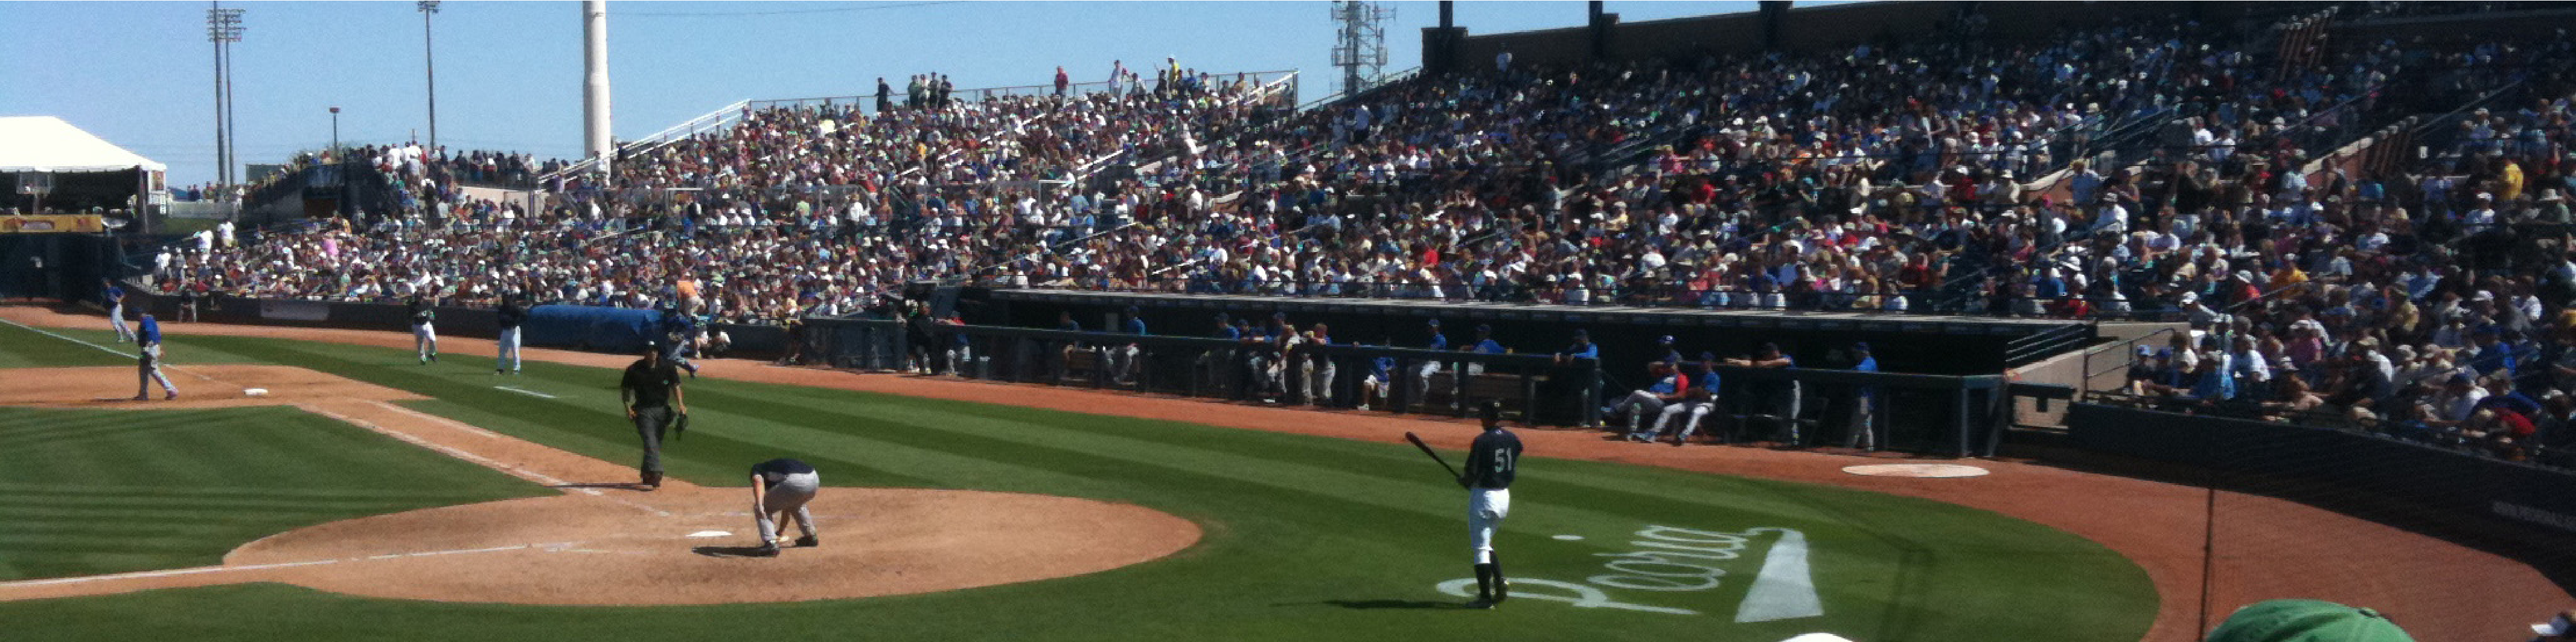
\includegraphics[width=\textwidth]{figures/sampleteaser}
 % \caption{Seattle Mariners at Spring Training, 2010.}
 % \Description{Enjoying the baseball game from the third-base
 % seats. Ichiro Suzuki preparing to bat.}
 % \label{fig:teaser}
%\end{teaserfigure}

%%
%% This command processes the author and affiliation and title
%% information and builds the first part of the formatted document.
\maketitle

\section{Introduction}

\section{Previous Work}

\section{CircusTent}

\begin{figure*}[!t]
\centering
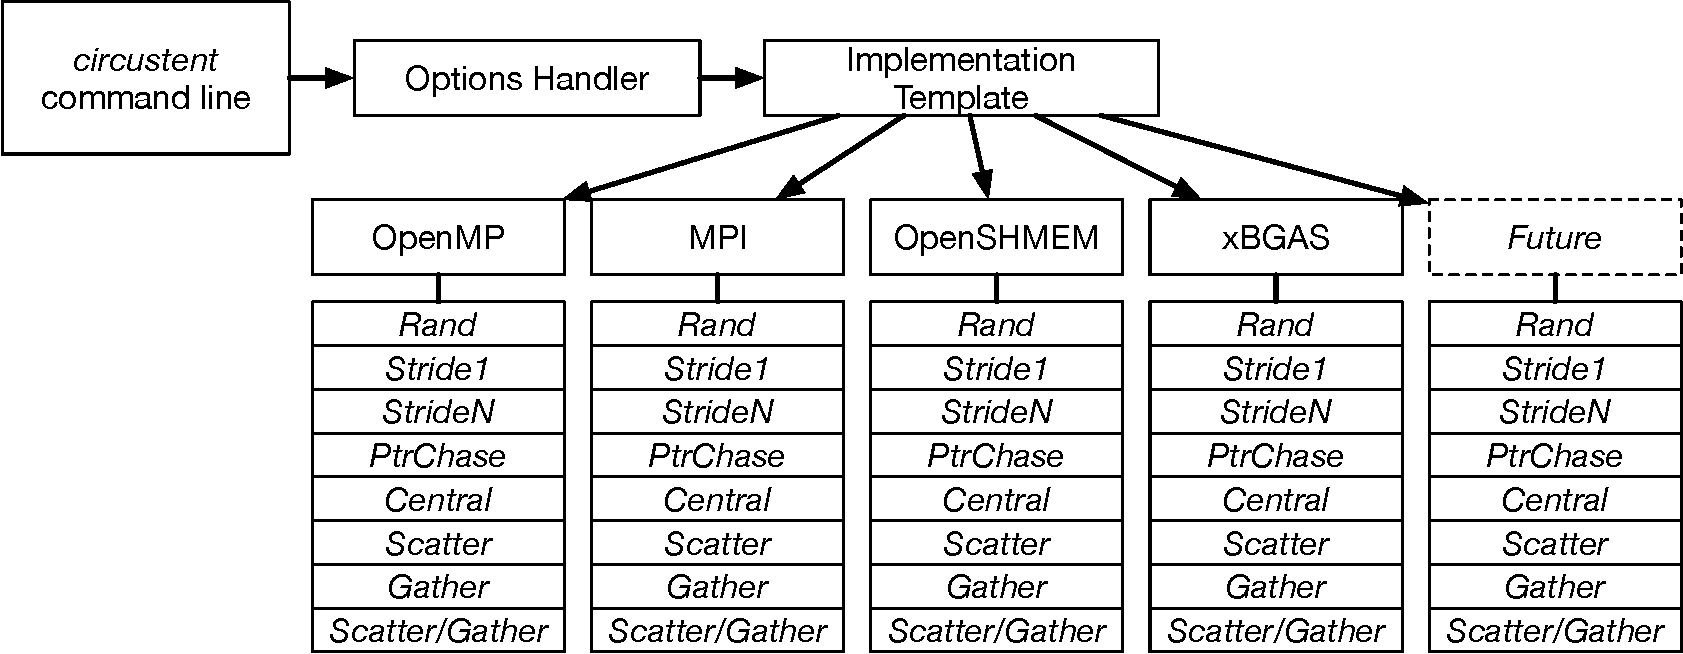
\includegraphics[width=5in]{figures/arch.pdf}
\caption{CircusTent Architecture}
\label{fig:ct_arch}
\end{figure*}

\subsection{Benchmark Overview}

\subsection{Programming Models}

\subsection{Algorithms}

The CircusTent infrastructure contains eight individual benchmark kernels.  Each 
kernel is described in terms of a generic atomic operation, \textit{AMO}.  However, 
each kernel may be implemented using any platform-supported 
atomic operations.  In the case of this study, we utilize atomic \textit{Add} 
and atomic \textit{Compare-and-Swap} (CAS) operations to implement 
each kernel, respectively.  

The first kernel is a basic random access kernel (Algorithm~\ref{alg:1}).  The kernel 
allocates two array structures.  The \texttt{VAL} array contains a series 
of values.  The \texttt{IDX} array contains a series of valid indices within 
the scope of the \texttt{VAL} array.  Prior to the execution of the kernel, the 
indices are randomly selected and written to the \texttt{IDX} array using a linear 
congruential randomizer.  For each iteration of the loop, a single \texttt{VAL} 
array entry is updated using an atomic operation.  In this manner, the random 
access kernel contains one memory load (\texttt{IDX[i]}) and one atomic operation for each iteration 
of the loop.  The goal of this kernel is to observe the performance of atomic operations 
when the platform has a limited ability to cache data for subsequent iterations.   

\begin{algorithm}
\SetAlgoLined
\For{$i\gets0$ \KwTo $iters$ \KwBy $1$}{
AMO(VAL[IDX[i]])
}
\caption{Random Access Kernel}
\label{alg:1}
\end{algorithm}

The second kernel encapsulates a simple, stride-1 kernel (Algorithm~\ref{alg:2}).  
The kernel allocates a single array (\texttt{VAL}) that contains a series of values.  
For each iteration of the loop, the kernel updates a single value in the array in linear 
fashion using a single atomic operation.  In this manner, a platform may utilize 
data prefetching and/or caching in order to optimize the access to data members 
in this kernel in an optimal manner similar in form to dense vectors or matrices.  

\begin{algorithm}
\SetAlgoLined
\For{$i\gets0$ \KwTo $iters$ \KwBy $1$}{
AMO(VAL[i])
}
\caption{Stride-1 Kernel}
\label{alg:2}
\end{algorithm}

The third kernel is similar in form to the second kernel.  In this kernel, 
we utilize the same \texttt{VAL} array structure as mentioned above, 
but we permit the user to define the unit stride by which we access the 
array (Algorithm~\ref{alg:3}).  
For example, if the user seeks to determine what the raw memory bandwidth is 
of parallel atomics by forcing every access to induce a cache line miss, the 
stride-n kernel can accomplish this.  Further, for each parallel PE participating 
in the kernel execution, the starting index is at least \textit{iters} distance from 
the previous PE.  

\begin{algorithm}
\SetAlgoLined
\For{$i\gets0$ \KwTo $iters$ \KwBy $stride$}{
AMO(ARRAY[i])
}
\caption{Stride-N Kernel}
\label{alg:3}
\end{algorithm}

The fourth 

\begin{algorithm}
\SetAlgoLined
\For{$i\gets0$ \KwTo $iters$ \KwBy $1$}{
start = AMO(IDX[start])
}
\caption{Pointer Chase Kernel}
\label{alg:4}
\end{algorithm}

\begin{algorithm}
\SetAlgoLined
\For{$i\gets0$ \KwTo $iters$ \KwBy $1$}{
AMO(ARRAY[0])
}
\caption{Central Kernel}
\label{alg:5}
\end{algorithm}

\begin{algorithm}
\SetAlgoLined
\For{$i\gets0$ \KwTo $iters$ \KwBy $1$}{
dest = AMO(IDX[i+1])\\
val = AMO(ARRAY[i])\\
AMO(ARRAY[dest], val) // ARRAY[dest] = val
}
\caption{Scatter Kernel}
\label{alg:6}
\end{algorithm}

\begin{algorithm}
\SetAlgoLined
\For{$i\gets0$ \KwTo $iters$ \KwBy $1$}{
dest = AMO(IDX[i+1])\\
val = AMO(ARRAY[dest])\\
AMO(ARRAY[i], val) // ARRAY[i] = val
}
\caption{Gather Kernel}
\label{alg:7}
\end{algorithm}

\begin{algorithm}
\SetAlgoLined
\For{$i\gets0$ \KwTo $iters$ \KwBy $1$}{
src = AMO(IDX[i])\\
dest = AMO(IDX[i+1])\\
val = AMO(ARRAY[src])\\
AMO(ARRAY[dest], val) // ARRAY[dest] = val
}
\caption{Scatter/Gather Kernel}
\label{alg:8}
\end{algorithm}

We summary the number of atomic operations required 
to perform each kernel in Table~\ref{tab:amodistro}.  However, 
this may vary depending upon how each platform implements 
a respective atomic operation.  The CircusTent implementation 
infrastructure supports the ability to override these defaults for 
each platform/programming model.    

\begin{table}
  \caption{Atomic Operation Distribution}
  \label{tab:amodistro}
  \begin{tabular}{cc}
    \toprule
    Benchmark&AMOs Per Iteration\\
    \midrule
   Rand & 1\\
   Stride-1 & 1\\
   Stride-N & 1\\
   Pointer Chase & 1\\
   Central & 1\\
   Scatter & 3\\
   Gather & 3\\
   Scatter/Gather & 4\\
  \bottomrule
\end{tabular}
\end{table}

\subsection{Normalizing the Results}
\label{sec:normalizingtheresults}

Given the native extensibility of CircusTent to 
support a multitude of programming models and 
platforms, we seek to develop a normalized metric such that 
we can compare results across platforms and differing degrees 
of execution parallelism.  For this, we introduce the \textit{GAMs} 
metric.  

The \textit{GAMs}, or \textit{billions of atomic operations per second}, 
metric encapsulates the number of parallel execution elements (\textit{PE}), the atomic 
operation algorithmic complexity and the wall clock execution time in a single 
metric.  As we see in Equation~\ref{eq:gams}, the metric is a ratio of the total 
number of atomic operations executed for all parallel parallel execution elements 
(in billions) across all iterations and the wall clock execution time.  The atomic operation 
algorithmic complexity is the total number of atomic operations required for a single 
\textit{PE} to execute a single iteration of the target CircusTent kernel.  This is equivalent 
to the \textit{AMOs Per Iteration} column in Table~\ref{tab:amodistro}.  

\begin{equation}
\label{eq:gams}
  GAMs = \frac{(PEs \times Iters \times AMOs\_Per\_Iter)/1e^{9}}{time}
\end{equation}

\section{Benchmark Evaluation}

\subsection{Methodology}

\begin{table*}
\caption{Benchmark System Configurations}
\label{tab:benchsys}
\begin{tabular}{cccccccc}
\toprule
System&Clock&Threads/Socket&Sockets&Cache/Socket&MemSize&OS&Compiler\\
\midrule
Xeon-X5650&2.67Ghz&6&2&12MiB&64GiB&Ubuntu 18.04 4.15.0-88 & GCC 7.5.0\\
Xeon-X5620&2.4Ghz&6&2&12MiB&48GiB&Ubuntu 16.04 4.4.0-87 & GCC 5.4.0\\
Core i5-3210M&2.5Ghz&4&1&3MiB&4GiB&macOS 10.13.6&clang 9.1.0\\
Opteron 4130&800Mhz&4&2&512MiB&64GiB&Centos7 3.10.0-957.12.1&GCC 8.3.1\\
Cortex-A72&1.5Ghz&4&1&1MiB&4GiB&NNN&NNN\\
Cortex-A53&1.4Ghz&4&1&64KiB&512MiB&NNN&NNN\\
Xeon-E5-2620&2.6Ghz&12&1&16MiB&64GiB&Ubuntu 16.04 4.4.0-164&GCC 5.4.0\\
Xeon-E5-2670&2.5Ghz&10&2&24MiB&NNN&Centos7 3.10.0&GCC 7.3.0\\
Xeon-E5-2695&2.10Ghz&36&2&48MiB&192GiB&Centos7 NNN&NNN\\
i7-3930K&3.20Ghz&12&1&12MiB&64GiB&Linux Mint 18.3 NNN&NNN\\
i7-4980HQ&2.80Ghz&8&1&16MiB&16GiB&macOS 10.15.3&GCC 9.2.0\\
Ryzen V1605B&1.4Ghz&8&1&512KiB&32GiB&Ubuntu 19.04 5.2.10&GCC 8.3.0\\
Xeon Phi 7250&1.40Ghz&272&1&1MiB&16GiB&SLES 4.12.14&GCC 8.3.0\\
Xeon E5-2698&2.30Ghz&32&2&40MiB&128GiB&SLES 4.12.14&GCC 8.3.0\\
\bottomrule
\end{tabular}
\end{table*}

\subsection{Results}

\begin{figure}[!t]
\centering
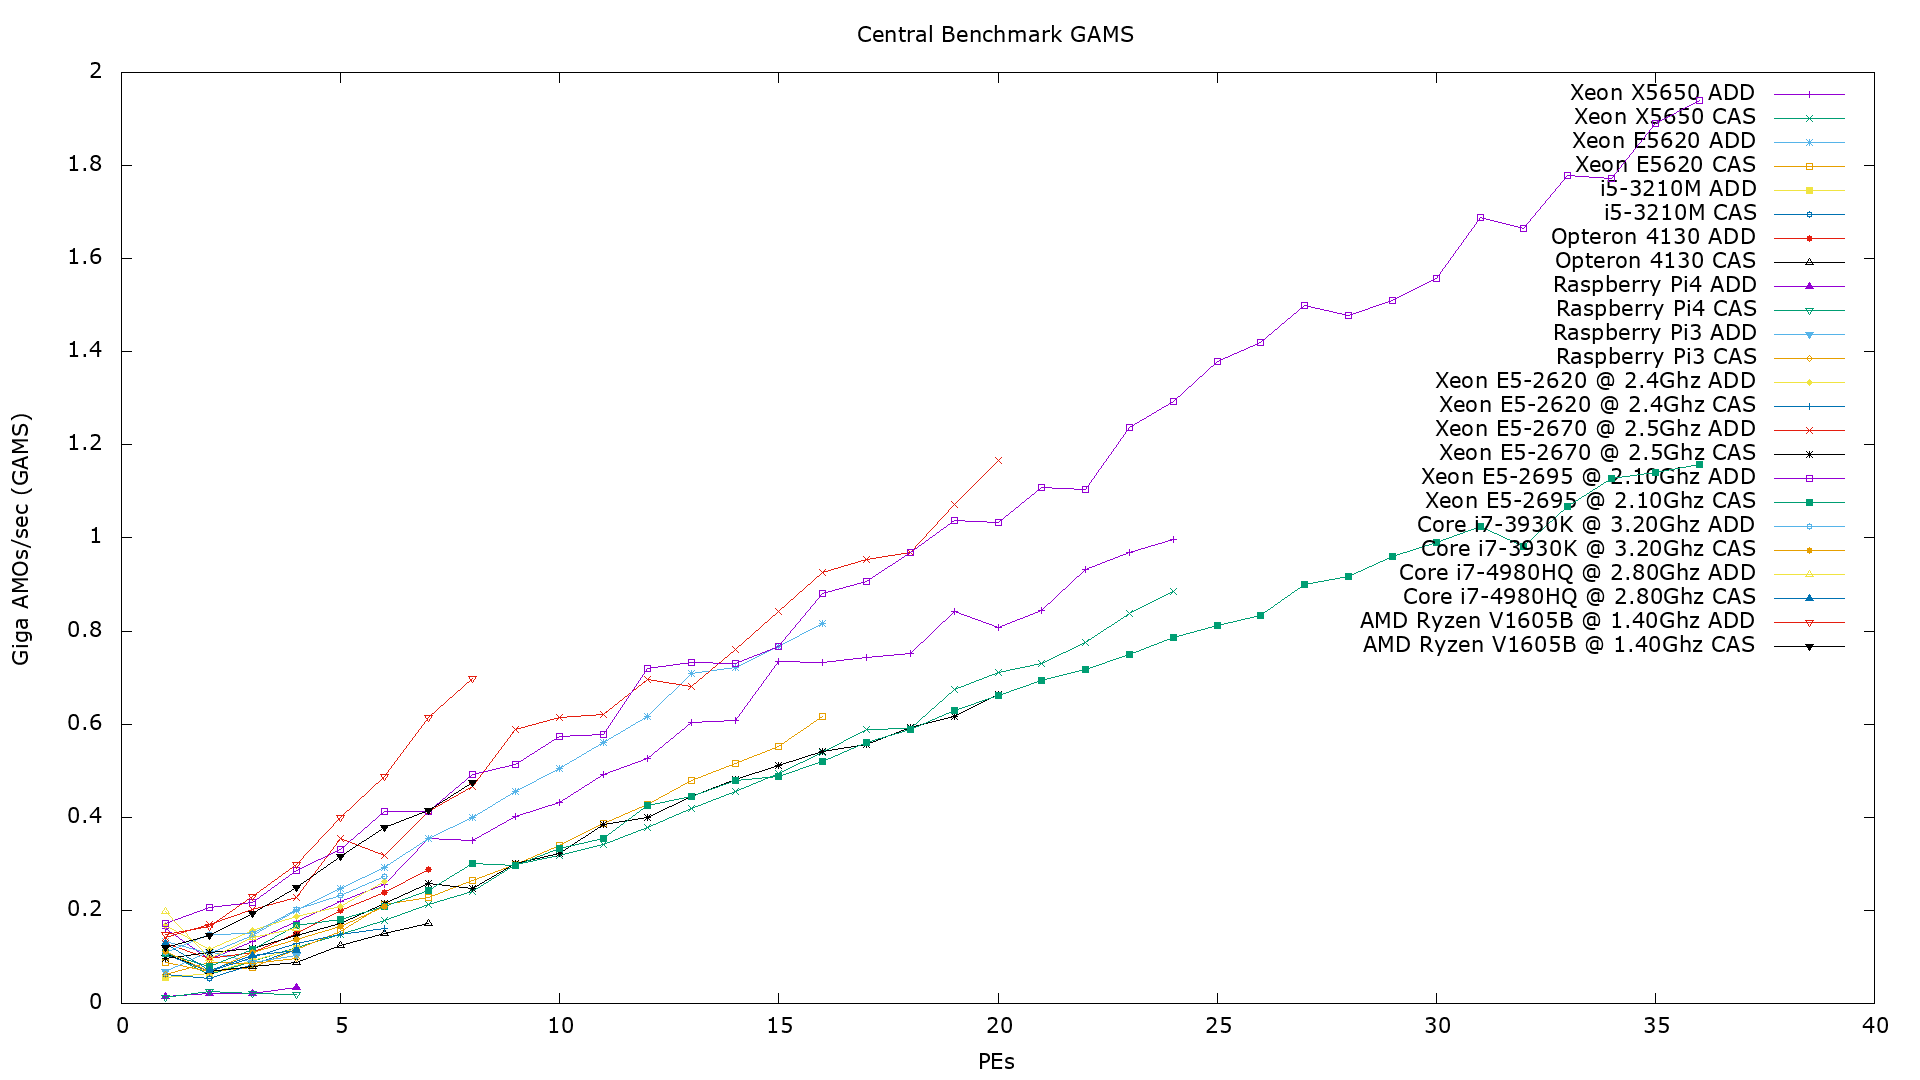
\includegraphics[width=3.5in]{figures/CENTRAL_GAMS.png}
\caption{Central Benchmark GAMS}
\label{fig:central_gams}
\end{figure}

\begin{figure}[!t]
\centering
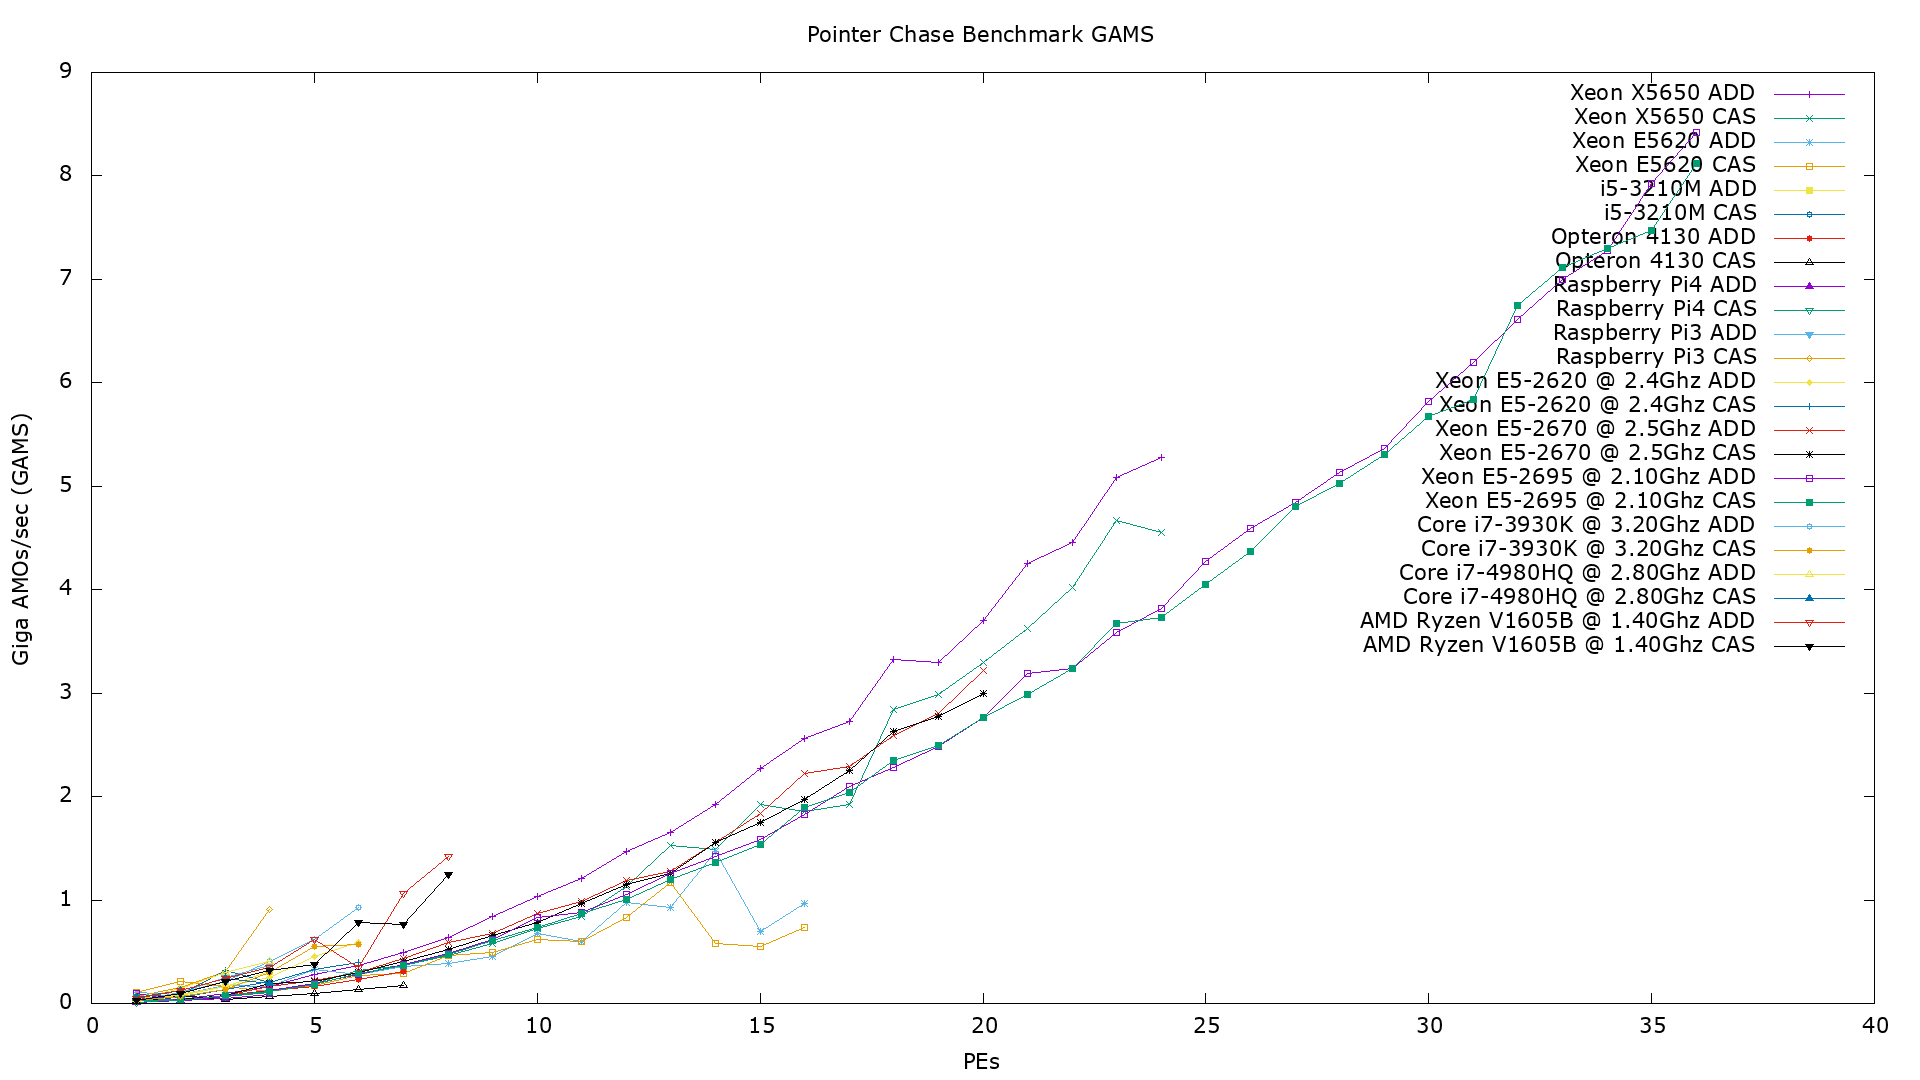
\includegraphics[width=3.5in]{figures/PTRCHASE_GAMS.png}
\caption{Pointer Chase Benchmark GAMS}
\label{fig:ptrchase_gams}
\end{figure}

\begin{figure}[!t]
\centering
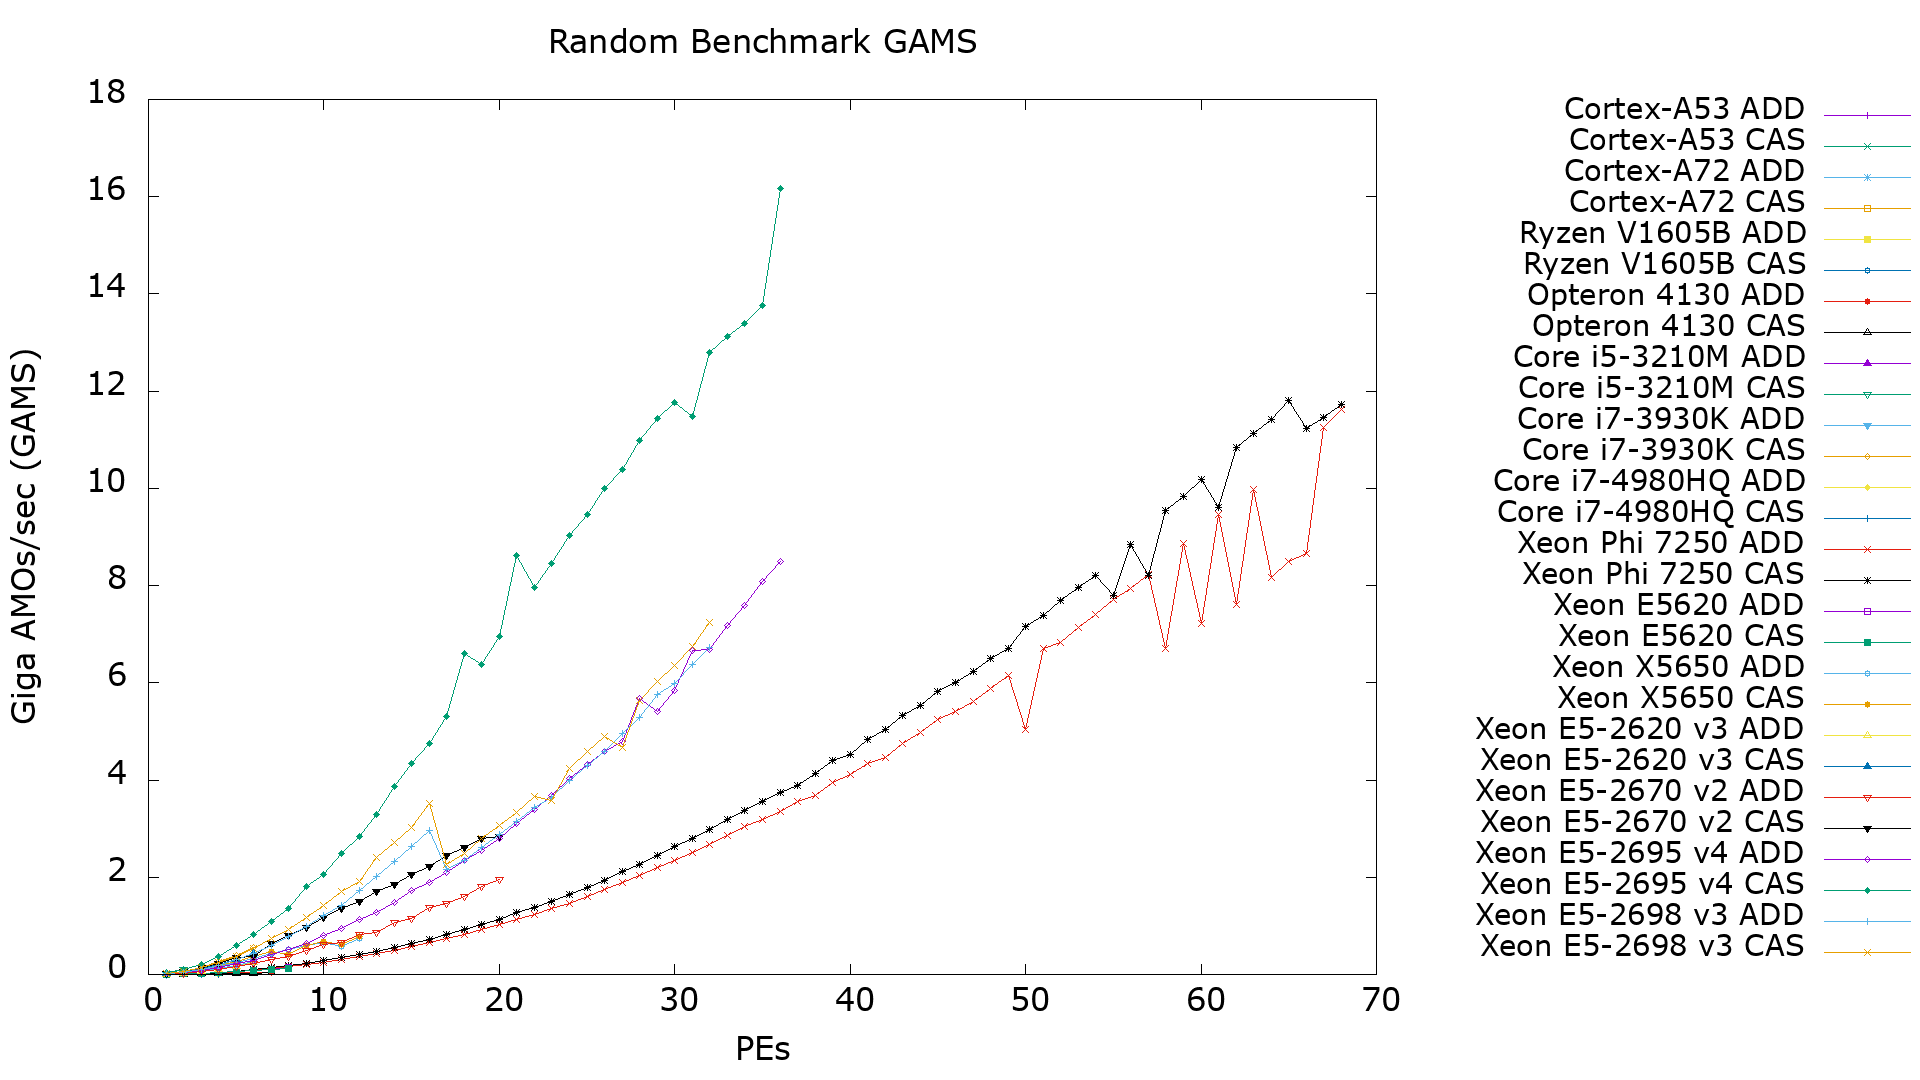
\includegraphics[width=3.5in]{figures/RAND_GAMS.png}
\caption{Random Benchmark GAMS}
\label{fig:rand_gams}
\end{figure}

\begin{figure}[!t]
\centering
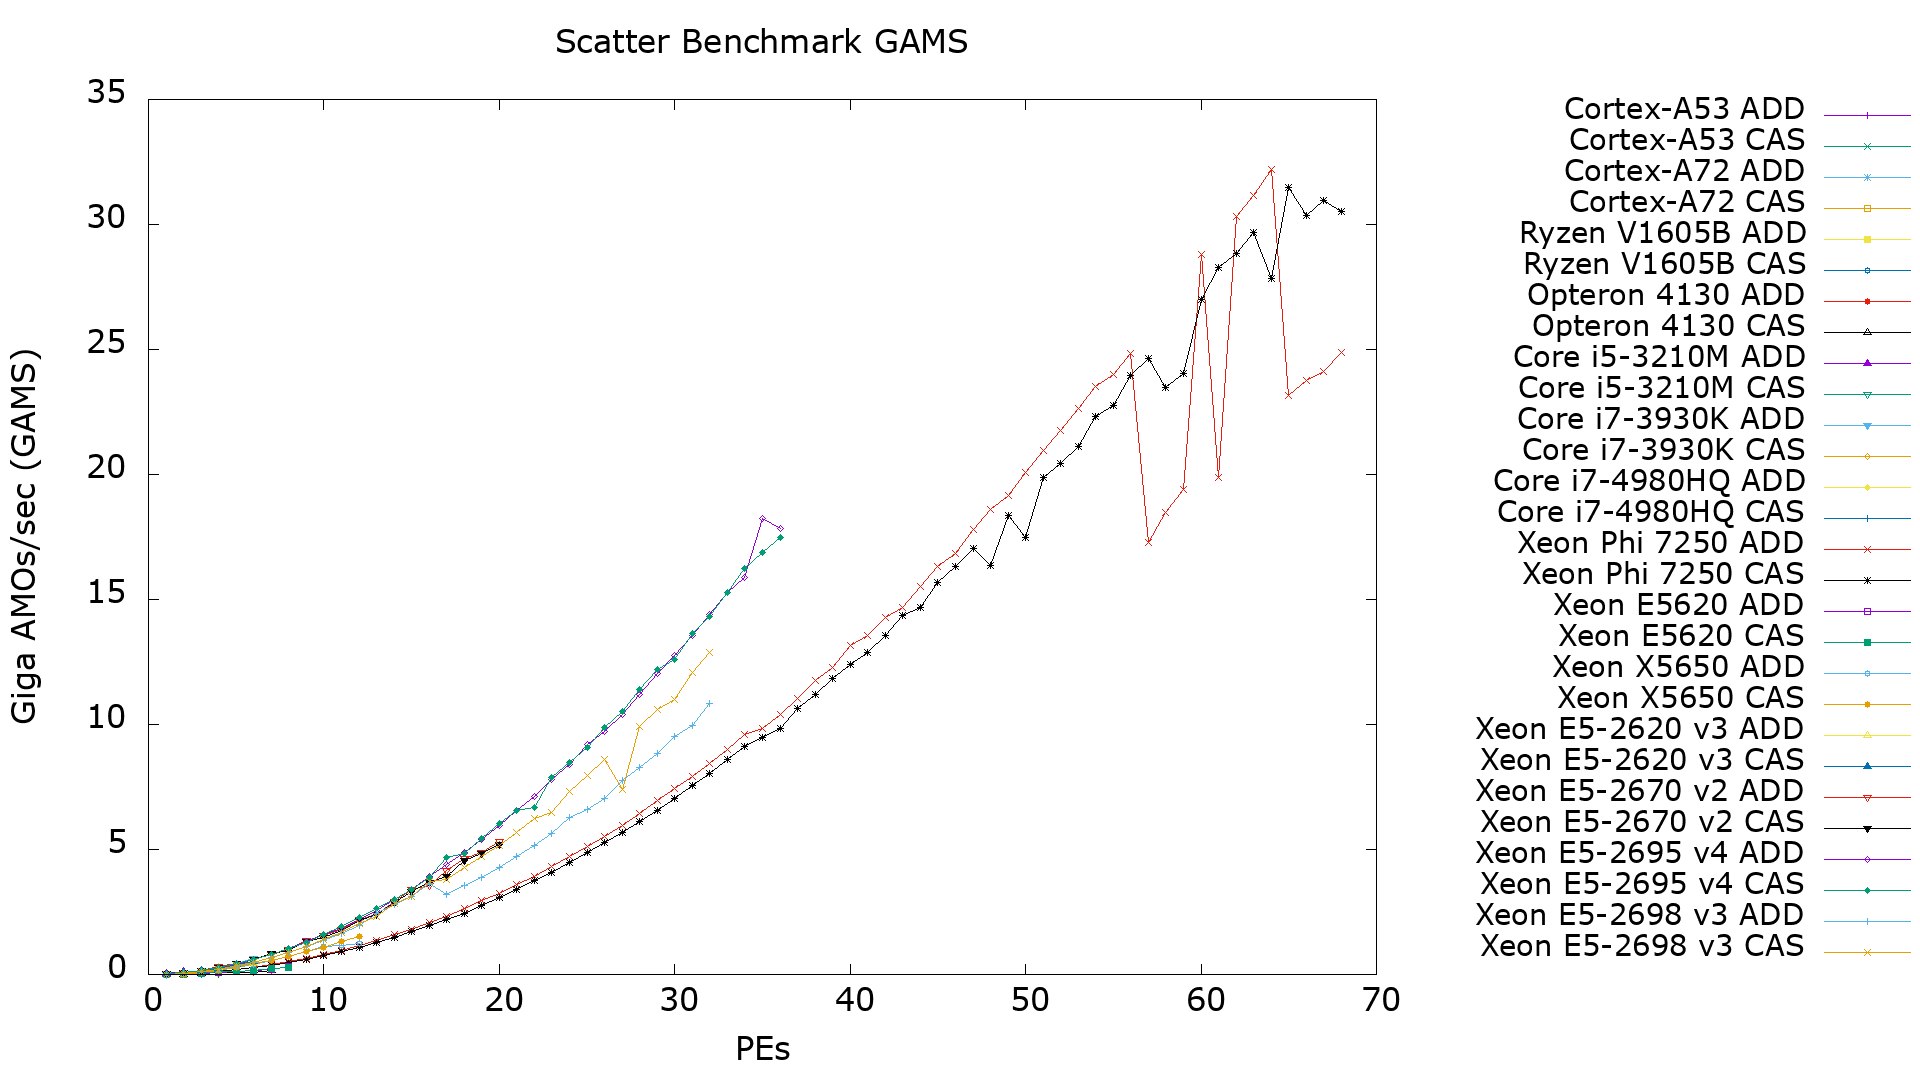
\includegraphics[width=3.5in]{figures/SCATTER_GAMS.png}
\caption{Scatter Benchmark GAMS}
\label{fig:scatter_gams}
\end{figure}

\begin{figure}[!t]
\centering
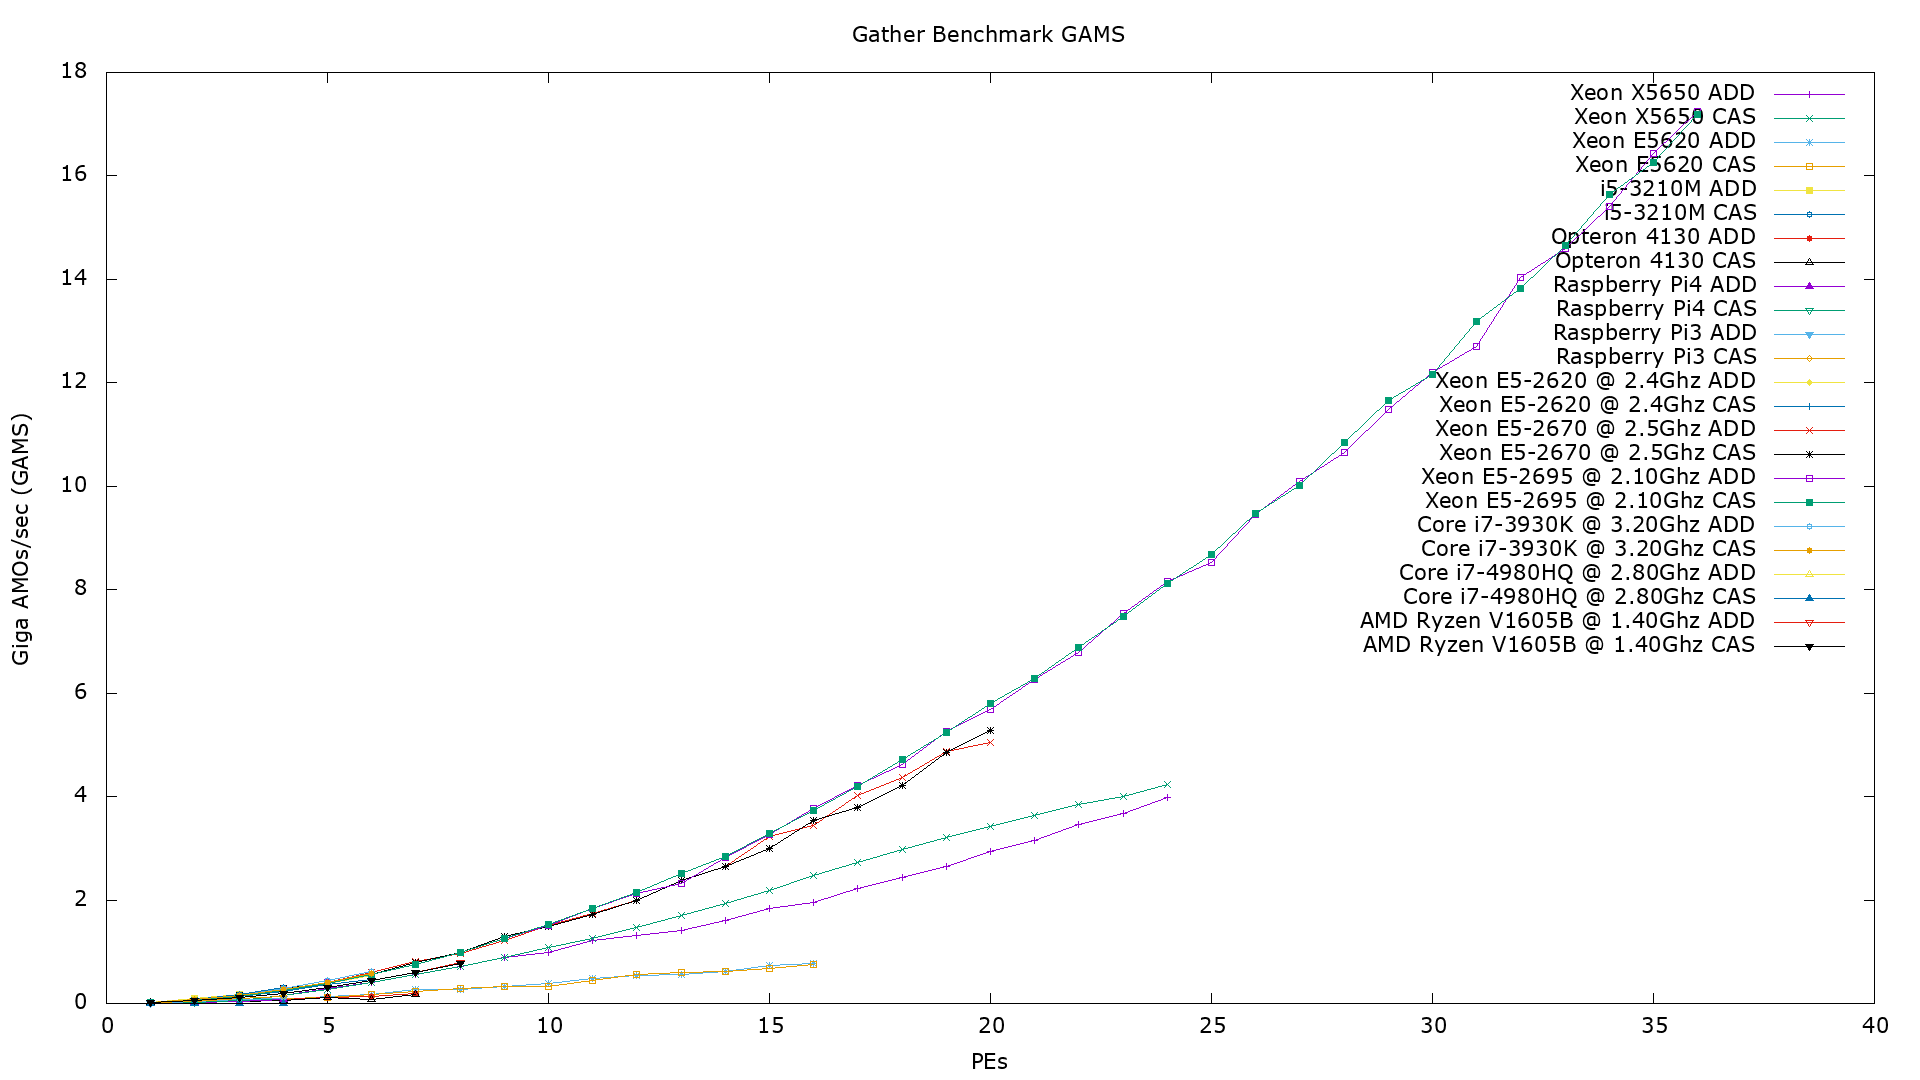
\includegraphics[width=3.5in]{figures/GATHER_GAMS.png}
\caption{Gather Benchmark GAMS}
\label{fig:gather_gams}
\end{figure}

\begin{figure}[!t]
\centering
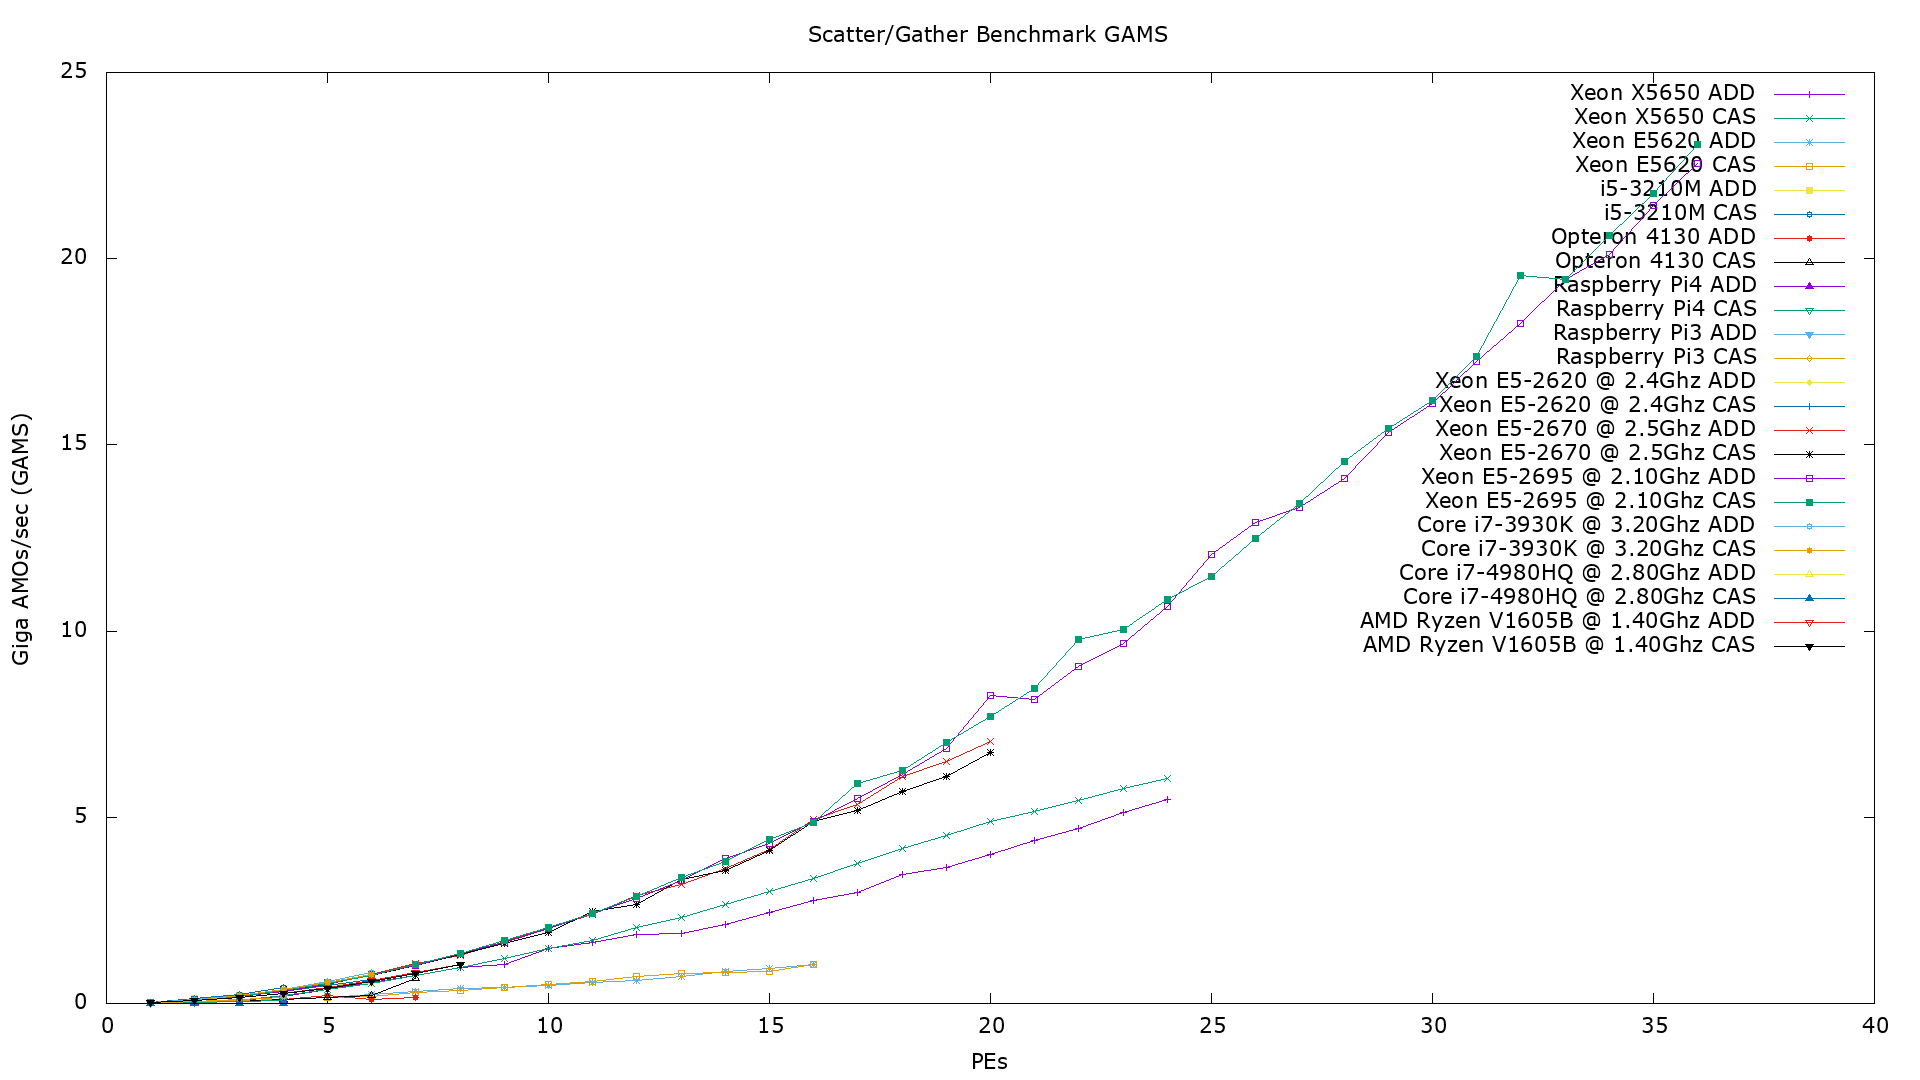
\includegraphics[width=3.5in]{figures/SG_GAMS.png}
\caption{Scatter/Gather Benchmark GAMS}
\label{fig:sg_gams}
\end{figure}

\begin{figure}[!t]
\centering
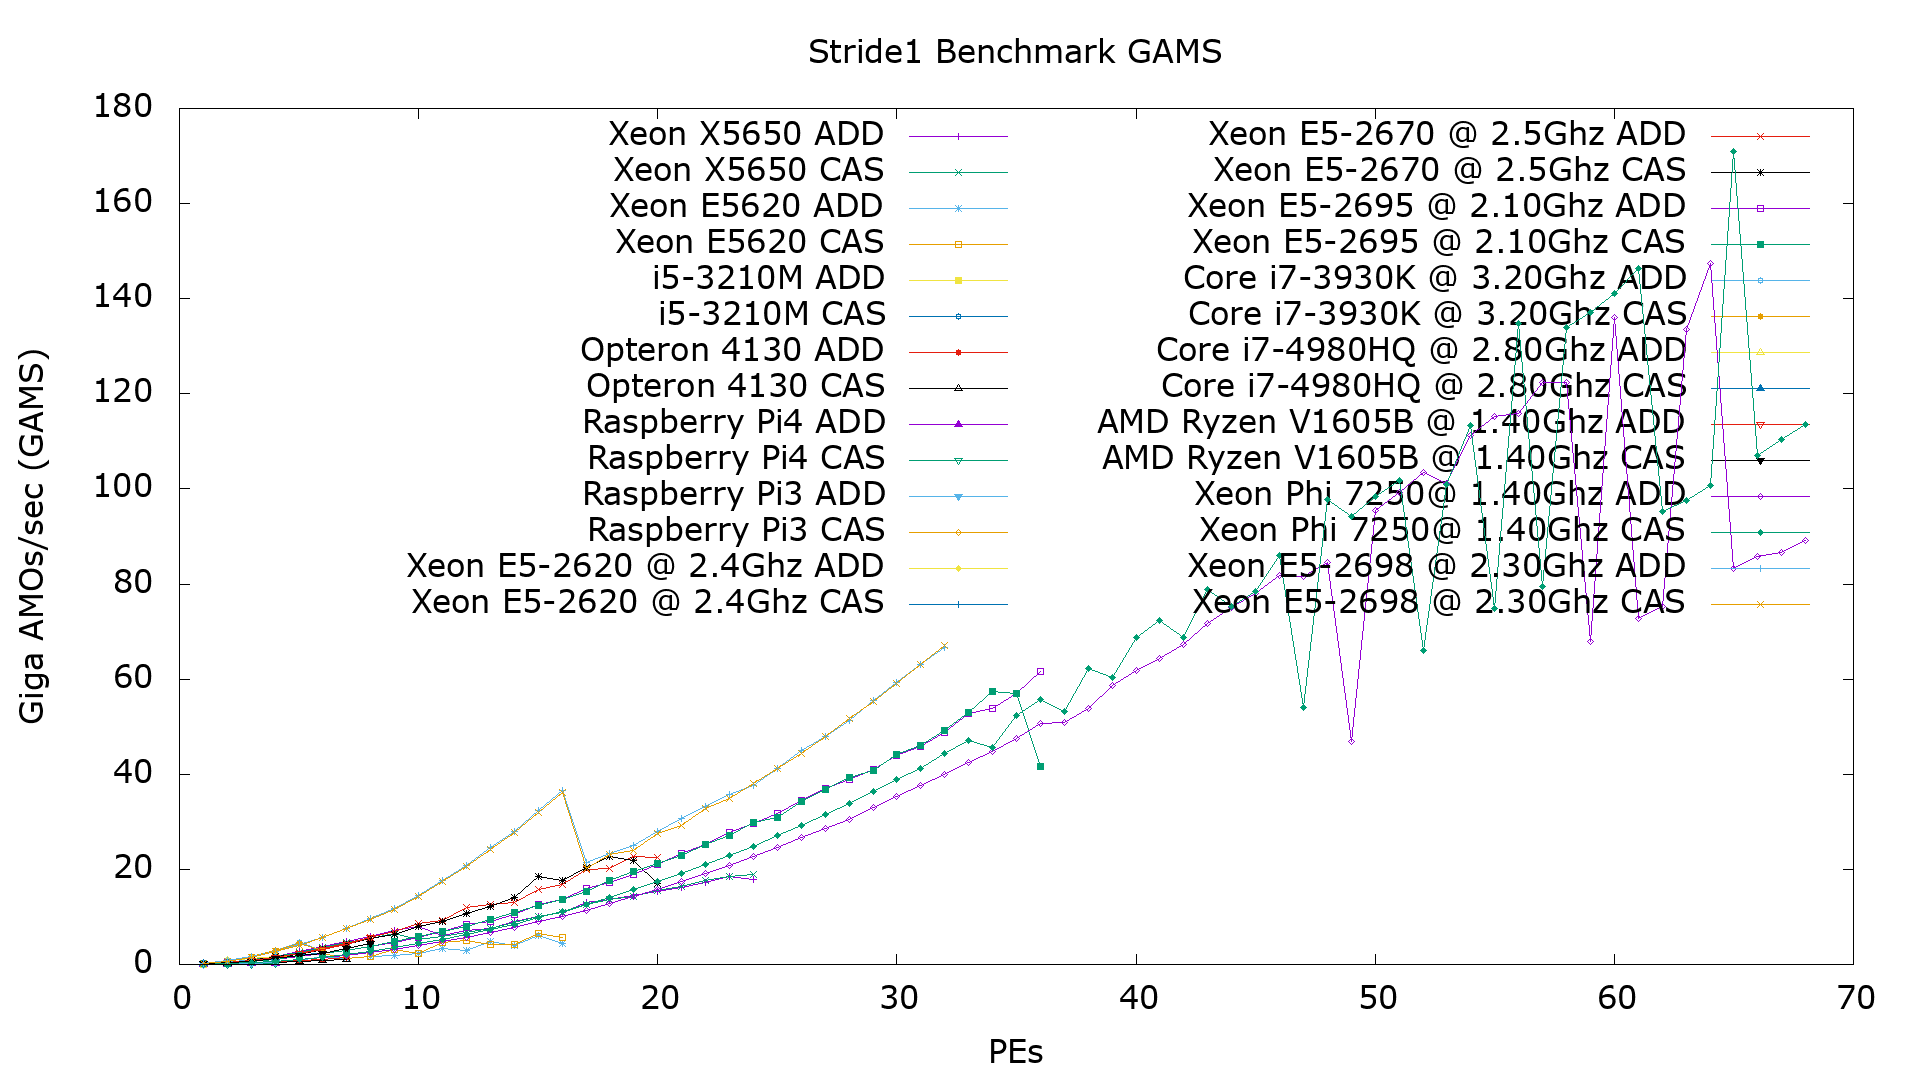
\includegraphics[width=3.5in]{figures/STRIDE1_GAMS.png}
\caption{Stride-1 Benchmark GAMS}
\label{fig:s1_gams}
\end{figure}

\begin{figure}[!t]
\centering
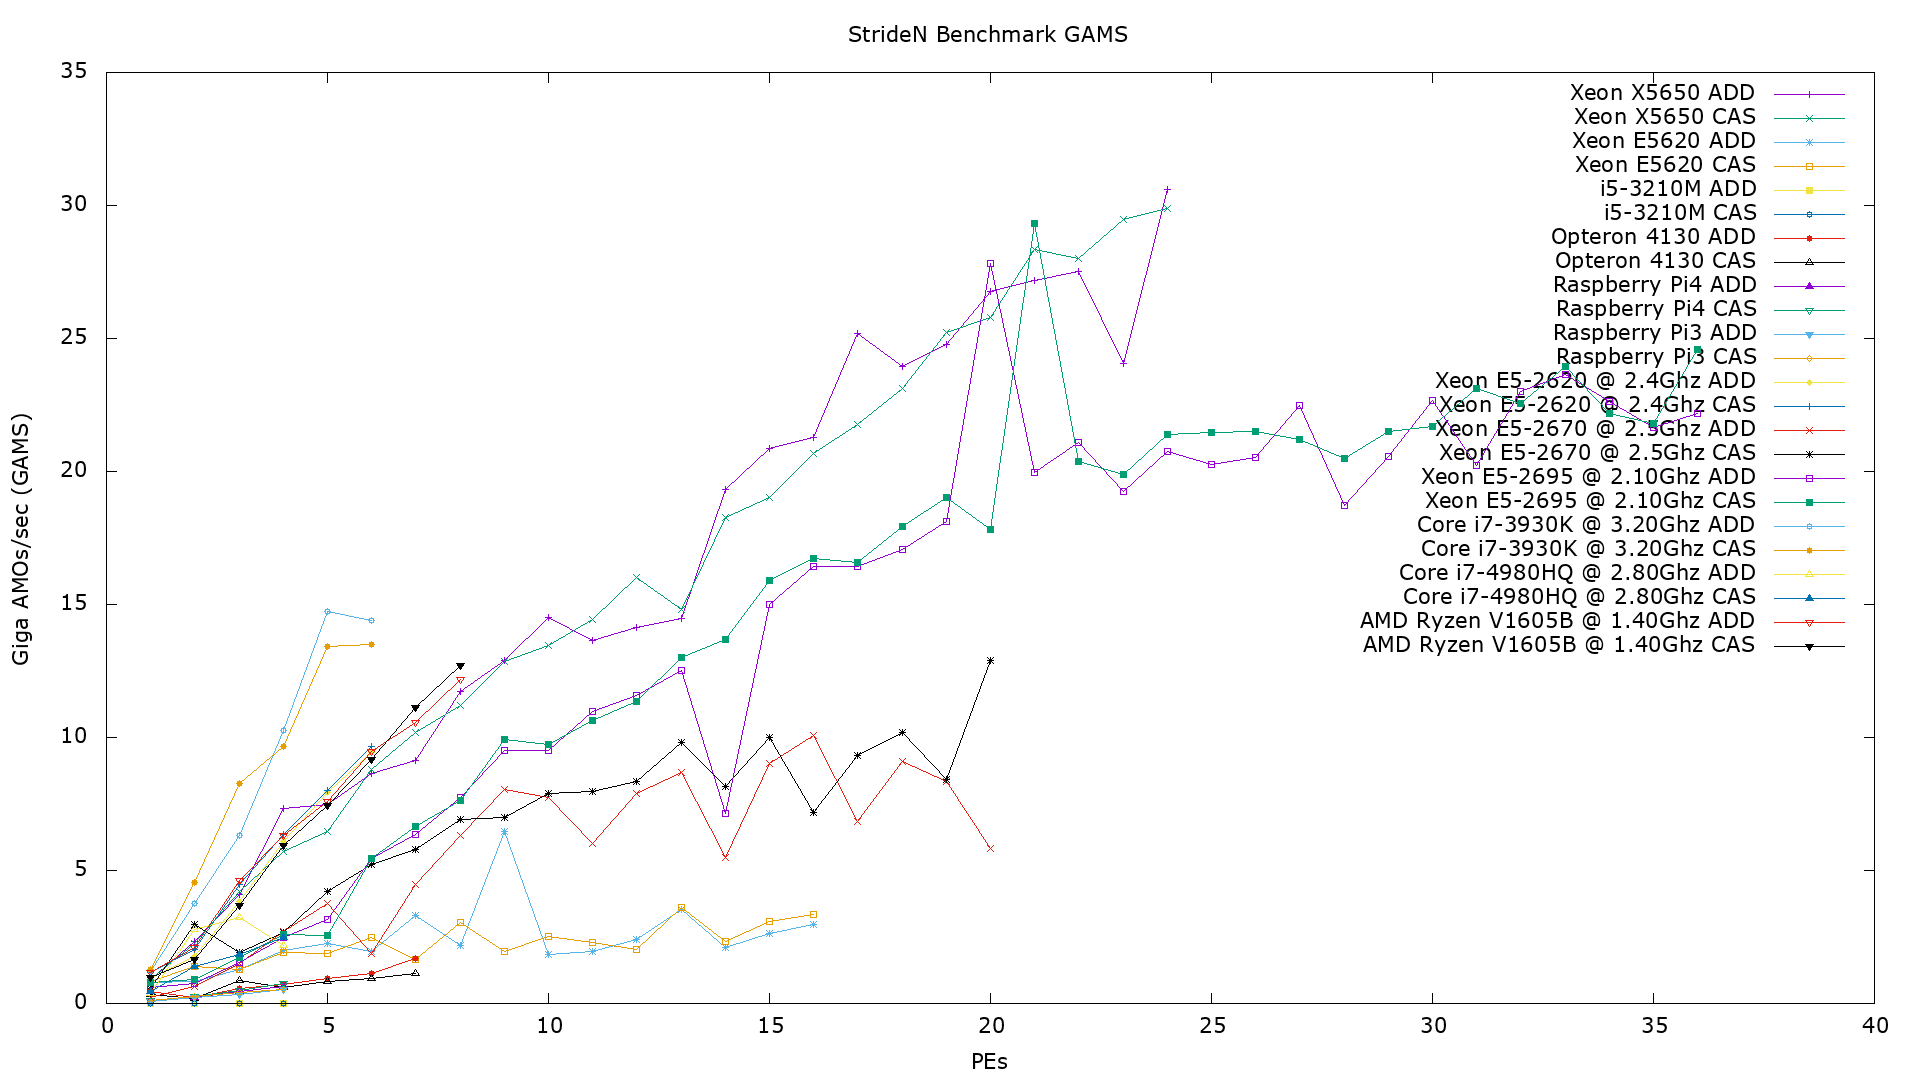
\includegraphics[width=3.5in]{figures/STRIDEN_GAMS.png}
\caption{Stride-N Benchmark GAMS}
\label{fig:sn_gams}
\end{figure}

\section{Conclusions}

\section{Future Work}

this is a reference~\cite{lavin2018spatter}

\begin{acks}
Research reported in this publication was supported by the U.S. Department of Defense
under Contract FA8075$-$14$-$D$-$0002.
\end{acks}

%---- END CTPAPER

%%
%% The next two lines define the bibliography style to be used, and
%% the bibliography file.
\bibliographystyle{ACM-Reference-Format}
\bibliography{sample-base}

\end{document}
\endinput
%%
%% End of file `sample-sigconf.tex'.
